\section{Auswertung}
\label{sec:Auswertung}

\subsection{Bestimmung einer Ausgleichskurve}
\begin{figure}
  \centering
  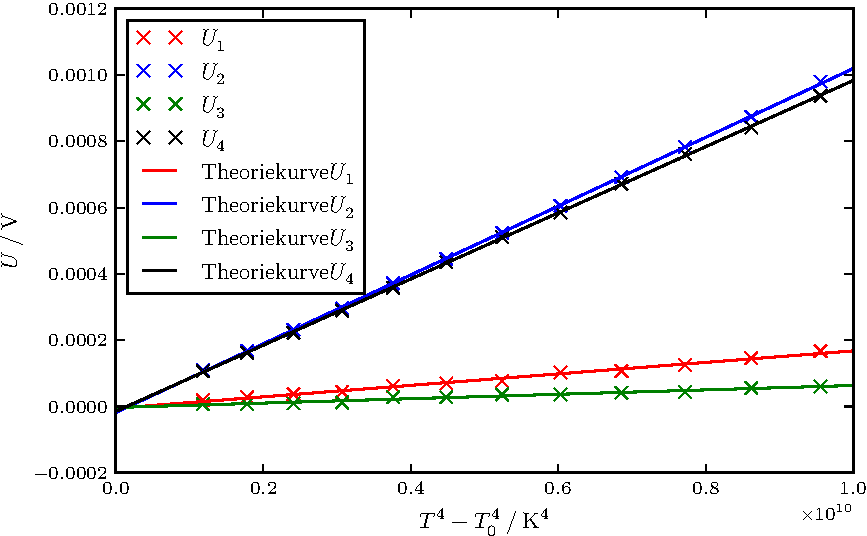
\includegraphics{plot.pdf}
  \caption{Plot.}
  \label{fig:plot}
\end{figure}
Die gemessenen Daten für die Tempeatur $T_1$ des wärmeren sowie die Temperatur
$T_2$ des kälteren Reservoirs wurden gegen die Zeit $t$ in Minuten abgetragen.
Mithilfe von SciPy wurde jeweils eine Ausgleichskurve für die folgende Funktion
berechnet:
\begin{equation}
  T(t)=A \cdot t^2 + B \cdot t + C
\end{equation}
Die Parameter $A$, $B$ und $C$ wurden bestimmt zu
\begin{align*}
A_{T_1} &= \SI{-3.87601 +- 0.10382e-6}{\kelvin\per\second²} \\
B_{T_1} &= \phantom{1}\SI{0.02345 +- 0.00019}{\kelvin\per\second} \\
C_{T_1} &= \phantom{1}\SI{293.592 +- 0.062}{\kelvin} \\
A_{T_2} &= \phantom{1}\SI{4.34879 +- 0.08533e-6}{\kelvin\per\second²}  \\
 B_{T_2} &= \SI{-0.01815 +- 0.00016}{\kelvin\per\second} \\
  C_{T_2} &= \phantom{1}\SI{294.936 +- 0.062}{\kelvin}
\end{align*}

Durch Ableiten und Einsetzen in die Ausgleichskurve
\begin{equation}
  \frac{\symup{d}T}{\symup{d}t}= 2 \cdot A \cdot t + B
\end{equation}
erhält man folgende Werte der Differentialquotienten:
\begin{table}
  \centering
  \caption{Differentialquotienten}
  \label{tab:tabelle1}
  \sisetup{table-format=1.2}
  \begin{tabular}{c c c c c}
    \toprule
    {$t [\si{\second}]$} & {$T_1 [\si{\kelvin}]$} & {$T_2 [\si{\kelvin}]$} & {$\frac{\symup{d}T_1}{\symup{d}t} [\si{\kelvin\per\second}]$}  & {$\frac{\symup{d}T_2}{\symup{d}t} [\si{\kelvin\per\second}]$}\\
    \midrule
    \num{420} & \num{29.6 +- 0.1} & \num{14.9 +- 0.1} & \num{0.021954 +- 0.000212} & \num{-0.014500 +- 0.000174} \\
    \num{840} & \num{37.5 +- 0.1} & \num{19.5 +- 0.1} & \num{0.016940 +- 0.000260} & \num{-0.010846 +- 0.000214} \\
    \num{1260} & \num{43.7 +- 0.1} & \num{5.7 +- 0.1} & \num{0.013684 +- 0.000325} & \num{-0.007193 +- 0.000267} \\
    \num{1680} & \num{48.9 +- 0.1} & \num{3.5 +- 0.1} & \num{0.010428 +- 0.000399} & \num{-0.003988 +- 0.000328} \\
    \bottomrule
  \end{tabular}
\end{table}
\\
Für die Fehlerrechnung wurde bei der vorliegenden Rechnung und bei allen folgenden Rechnungen das Gauß\'sche Fehlerfortpflanzungsgesetz
\begin{equation}
\increment{f} = \sqrt{(\frac{\partial f}{\partial x_1}\increment{x_1})^2 + (\frac{\partial f}{\partial x_2}\increment{x_2})^2 + \dotsc + (\frac{\partial f}{\partial x_n}\increment{x_n})^2}
\end{equation}
für eine Funktion $f(x_1,x_2, \dotsc ,x_n)$ bei denen die Größen $x_1, x_2, \dotsc , x_n$ voneinander unabhängig sind.

\subsection{Güteziffervergleich}
Für eine ideale Wärmepumpe gilt
\begin{equation}
  v_{ideal} = \frac{T_1}{T_1-T_2}.
\end{equation}
Für die reale Wärmepunpe gilt jedoch die Formel
\begin{equation}
  v_{real}= \frac{\symup{d} Q_1}{\symup{d} tN} = (m_1c_w+m_kc_k)\frac{\symup{d} T_1}{\symup{d} tN}.
\end{equation}
wobei $ N = $ die Kompressorleistung, $ m_1$ die Masse des Wassers in $ R_1 $, $m_k$ die Masse des zu heizenden Reservoirs inklusive Kupferrohre, $ c_w $ die spezifische Wärmekapazität des Wassers sowie $ c_k $ die spezifische Wärmekapazität des Reservoirs und der Kuperrohre ist.
Da bei der Durchführung des Versuches \SI{4}{\litre} Wasser für $R_1$ verwendet wurden, berechnet sich $m_1$ zu $m_1 = \rho_{H_2O} \cdot V = \SI{4176.48}{\kilogram}$, wobei der Werte für $\rho_{H_20}$ der Literatur entnommen wurde.
Das Produkt aus $m_k$ und $c_k$ wurde vom Versuchsaufbau zu $\SI{750}{\joule\per\kelvin}$ abgelesen, $c_w$ wurde ebenfalls der Literatur zu $\SI{4,1819}{\kilo\joule\per\kilogram\kelvin}$ entnommen.
Die Kompressorleistung ergibt sich aus dem arithmetischen Mittelwert der Messdaten zu $N=124.77$.
Für die Differenzenquotienten wurden die Werte der Ausgleichskurve, angegeben in Tabelle 1 verwendet.

\begin{table}
  \centering
  \caption{Güteziffervergleich}
  \label{tab:tabelle1}
  \sisetup{table-format=1.2}
\begin{tabular}{c c c c c c c}
  \toprule
  {$t [\si{\second}]$} & {$T_1 [\si{\kelvin}]$} & {$T_2 [\si{\kelvin}]$} & {$\increment{T} [\si{\kelvin}]$} & {$v_{real, T_1}$}  & {$v_{real, T_2}$} & {$v_{ideal}$}\\
  \midrule
  \num{420} & \num{29.6 +- 0.1} & \num{14.9 +- 0.1} & \num{14.7 +- 0.1} & \num{2.948 +- 0.039} & \num{-2.117 +- 0.031} & \num{20.599 +- 0.193} \\
  \num{840} & \num{37.5 +- 0.1} & \num{19.5 +- 0.1} & \num{18.0 +- 0.1} & \num{2.473 +- 0.043} & \num{-1.584 +- 0.034} & \num{11.096 +- 0.054}  \\
  \num{1260} & \num{43.7 +- 0.1} & \num{5.7 +- 0.1} & \num{38.0 +- 0.1} & \num{1.998 +- 0.050} & \num{-1.050 +- 0.040} & \num{8.339 +- 0.029}  \\
  \num{1680} & \num{48.9 +- 0.1} & \num{3.5 +- 0.1} & \num{45.4 +- 0.1} & \num{1.522 +- 0.059} & \num{-0.517 +- 0.048} & \num{7.095 +- 0.021}  \\
  \bottomrule
\end{tabular}
\end{table}
Es fällt auf, dass sich die reale Güteziffer deutlich von der idealen Güteziffer unterscheidet.
Gründe für diese Differenz werden im Kapitel Diskussion besprochen.
\subsection{Massendurchsatz}
